\newpage
\appendix
\chapter{Conservative remapping with the {\tt fracwgt} option}
\label{subsec_fracwgt}

When a coupling field is valid only on a fraction of the source cells (fractional source field), there are different interpretations about the destination field that should be obtained on the destination grid after conservative remapping. 

A {\bf destination scaled field}, i.e. the remapping of the original field multiplied by its valid fraction on each cell, ensures conservation when the full destination cell area of the target grid is considered. However, because of the source fractions, it can become nonphysically small. 

Another way to consider the problem is to calculate a {\bf destination normalized scaled field} that will be in the physical range of the original field. This {\bf destination normalized scaled field} will be valid only on a fraction of the target, the {\bf active destination surface} that can be calculated with the {\bf active destination surface coefficient}.

The new option {\tt fracwgt} in OASIS3-MCT\_6.0 allows to pass, in the source component as argument of the {\tt oasis\_put}, the active fraction of the source cells together with the source coupling field and to obtain, in the target component in the {\tt oasis\_get}, the {\bf destination normalized scaled field}. It also allows to calculate the {\bf active destination surface coefficient}.

For instantaneous fields, option {\tt fracwgt} is not essential as the user could get the {\bf active destination surface coefficient} simply with the conservative remapping of the source fraction field. He/she could then obtain the {\bf destination normalized scaled field} by applying the element-wise division of the {\bf destination scaled field} by the {\bf active destination surface coefficient}.

However, for accumulated or averaged fields, option {\tt fracwgt} is essential to obtain the {\bf destination accumulated
normalized scaled field} and the {\bf accumulated active destination surface coefficients}, as they cannot be calculated in the  models because of the non permutation of the time and remapping operations. 

An example of how to use the {\tt fracwgt} option is given in  {\tt /pyoasis/examples/13-test-fracwgt}. 
\section{Introduction}

Conservative remapping is relevant for physical fields representing a flux or a concentration. \\
We can think of energy fluxes ($W/m^2$), 
precipitation rates ($mm/m^2$), tracer concentrations (ppb or similar).\\
The remapping is required to:
\begin{enumerate}
    \item preserve the total energy or mass
    \item avoid abnormal local values of fluxes or concentrations

\end{enumerate}
In models with no sub-grid fractions, the surface integral quantity to be preserved is the sum of the area of the unmasked source cells times the field on the cell
\[\sum_iA_{Si}F_{Si}\]
where \(A_{Si}\) and \(F_{Si}\) are respectively the area and the field of the source cell \(i\).
A conservative remapping will grant that
\[\sum_iA_{Si}F_{Si} = \sum_jA_{Dj}F_{Dj}\]
where \(A_{Dj}\) and \(F_{Dj}\), the area and the field of the target cell \(j\), can be expressed as:
\[F_{Dj} = \sum_iw_{ij}F_{Si} \]
\[A_{Dj} = \sum_i\omega_{ij}A_{Si}\]
\(\omega_{ij}\), the fraction of the source cell \(i\) overlapping the destination cell \(j\), is related to the conservative remapping weight \(w_{ij}\) representing the area normalized fraction of the destination cell \(j\) intersected by the source cell \(i\) by, as in \cite{gmd-17-415-2024},:
\[w_{ij}=\omega_{ij}\frac{A_{Si}}{A_{Dj}}\]
Notice that, because of some assumptions on the representation of the cell edges on a sphere and to rounding errors, the \(A_{Dj}\) surface can slightly differ from the surface \(A^d_{Dj}\) prescribed in the destination model, but we will neglect this difference here. 

\section{What is a fractional field?}

For some models, a process represented on the model grid actually takes place only on a subset of it, whose boundaries are described at a finer resolution than the grid. The numerical translation of this choice is an extra mask-like field, providing the active (or unmasked) fraction \(f_i\in[0,1]\) for every cell.\\
The field is therefore described with values ranging in the usual physical valid interval (\emph{cf}. point 2. in the introduction), yet the integral quantity is scaled down to
\[\sum_iA_{i}f_iF_{i}\]
This scaling can be interpreted in two ways
\begin{enumerate}
    \item On cells with usual area \(A_i\), the flux is lowered to the {\bf scaled field} \(F^f_i=f_iF_i\)
    \item The flux \(F_i\), with values in the usual physical range, is active on a smaller {\bf active source surface} \(A^a_i = A_if_i\)

\end{enumerate}

\section{Instantaneous remapping}

When applying the conservative remapping on an instantaneous fractional source field (i.e. in OASIS jargon, no LOCTRANS or LOCTRANS/INSTANT time transformation), we grant the conservation of the scaled integral source quantity
\[\sum_iA_{Si}f_{Si}F_{Si}\]
Once again, we can use different interpretations.\\
If we consider that we are interpolating a {\bf scaled field} \(F^f_{Si}=f_{Si}F_{Si}\) with a standard conservative remapping,  and we are receiving the resulting 
{\bf destination scaled field}
\begin{equation}\label{eqn:inst_scaled}
    F^f_{Dj} = \sum_iw_{ij}f_{Si}F_{Si}
\end{equation}
then we will grant, as defined by the conservative remapping
\[\sum_iA_{Si}f_{Si}F_{Si} = \sum_jA_{Dj}F^f_{Dj}\]
where \(A_{Dj}\) is the full destination cell area. Yet the local values \(F^f_{Dj}\) could locally become nonphysically small.\\
%To overcome this issue, if we consider the conservative remapping weights in terms of ratios of active areas, we can redefine them as in
%\begin{equation}\label{wijprime}
%w'_{ij}=\omega_{ij}\frac{f_{Si}A_{Si}}{f^d_{Dj}A_{Dj}}=w_{ij}\frac{f_{Si}}{f^d_{Dj}}
%\end{equation}
It is now essential to define the {\bf active destination surface coefficients}, i.e. the active fraction of every destination cell, \(f_{Dj}\), with the conservative remapping of the source grid fractions: 
\begin{equation}\label{eqn:inst_dest_fract}
f_{Dj} = \sum_i{w_{ij}f_{Si}}
\end{equation}
 Using this coefficient \(f_{Dj}\), we can define a {\bf destination normalized scaled field} that will be in the physical range of the original field as
\begin{equation}\label{eqn:normalized_field}
F^{fn}_{Dj} = \frac{F^f_{Dj}}{f_{Dj}}    
\end{equation}
Note that if the active fraction of all source cells associated to one target cell \(f_{Si}\) are zero then both \(F^{f}_{Dj}\) and \(f_{Dj}\) are zero and equation \ref{eqn:normalized_field} becomes undefined. In that case, in OASIS3-MCT\_6.0, we set \(F^{fn}_{Dj}\) equal to zero.

In order to preserve the integral quantity we have to scale back the field:
\[\sum_iA_{Si}f_{Si}F_{Si} = \sum_jA_{Dj}f_{Dj}F^{fn}_{Dj}\]
For computing a conservative integral quantity on the destination side, the active destination surface coefficient \(f_{Dj}\) can be used to define the {\bf active destination surface} :
\begin{equation}\label{eqn:active_dest_area}
A^a_{Dj} = A_{Dj}f_{Dj}    
\end{equation}
so that
\[\sum_iA_{Si}f_{Si}F_{Si} = \sum_iA^a_{Si}F_{Si} =\sum_jA^a_{Dj}F^{fn}_{Dj}\]
Since OASIS3-MCT\_6.0, the {\tt oasis\_put} routine comes with an extra optional argument {\tt fracwgt}. If  the argument is present, it has to correspond to the active source fraction field \(f_S\), and the matching {\tt oasis\_get} will receive the normalized scaled field \(F^{fn}_D\). \\
Notice that for technical reasons, the active destination surface coefficient \(f_D\) cannot be recovered as an extra output of the {\tt oasis\_get} call. The user can recover it in two ways:
\begin{enumerate}
    \item send the active source fraction field \(f_S\) as a separate coupling field through a standard conservative remapping and directly get \(f_D\) (equation \ref{eqn:inst_dest_fract}) ; or
    \item compute the ratio between the destination scaled field and the destination normalized scaled field  
    \begin{enumerate}
    \item in the source model compute the scaled source field \(F^f_S = f_SF_S\)
    \item send this scaled field with a standard {\tt oasis\_put} call (i.e. without a {\tt fracwgt} argument) and on the destination side store the corresponding (non normalized) scaled field \(F^f_D\)
    \item send the (non scaled) source field \(F_S\) passing {\tt fracwgt}=\(f_S\) to the  {\tt oasis\_put} call and on the destination side store the corresponding normalized scaled field \(F^{fn}_D\) (equation \ref{eqn:normalized_field})
    \item compute the active destination surface coefficient as an element-wise division \(f_D = F^f_D \odot \frac{1}{F^{fn}_D}\)
    \end{enumerate}
\end{enumerate}
Once \(f_D\) is computed, the active destination surface to be used for computing integral quantities is finally obtained by scaling the destination cells surfaces \(A^a_D = A_D \odot f_D\)

Notice that it is mandatory that the treatments described in the namcouple for the two remappings b. and c. are strictly the same.

Even if the implementation of the first method is easier for instantaneous fields, we suggest using the second one that relies on the {\tt fracwgt} option because, as we will show in the following sections, it is compatible with time accumulated or time averaged remapping.\\\\


\section{Time accumulation}

Let's now consider the case in which the destination field has to be computed as the accumulation of remapped source fields at different times (i.e. in OASIS jargon, LOCTRANS/ACCUMUL time transformation)
\begin{equation}\label{destination_accumulatedblasoldcoeff}
F^+_{Dj}=\sum_t{\alpha F^t_{Dj}+\beta}=\sum_t{\alpha\left(\sum_i{w_{ij}F^t_{Si}}\right)+\beta}
\end{equation}

where \(\alpha\) and \(\beta\) are the coefficient of an affine transform that can be indicated with the {\tt BLASOLD} method. Because of the linearity of the operators we can neglect them in the following for the sake of readability. We therefore define the {\bf destination accumulated field} as
\begin{equation}\label{destination_accumulatedblasold}
F^+_{Dj}=\sum_t{F^t_{Dj}}=\sum_t{\sum_i{w_{ij}F^t_{Si}}}
\end{equation}

In the case where no subgrid fractions are used, the accumulating sum and the linear mapping can permute and we can easily obtain the {\bf destination accumulated field} as the remapping of the {\bf accumulated source fields}
\begin{equation}\label{destination_accumulated}
F^+_{Dj}=\sum_t{\sum_i{w_{ij}F^t_{Si}}} = \sum_i{w_{ij}\sum_t{ F^t_{Si}}}
\end{equation}
In that case, we can rewrite the conservative remapping as
\begin{equation} 
\sum_t{\sum_i{A_{Si}F^t_{Si}}} = \sum_t{\sum_j{A_{Dj}F^t_{Dj}}} = \sum_jA_{Dj}{\sum_t{F^t_{Dj}}} = \sum_j{A_{Dj}F^+_{Dj}}
\end{equation}
If we introduce a time varying fractional coefficient in the time accumulation equations, we can obtain the corresponding {\bf destination accumulated scaled field} by sending and remapping \(f^t_{Si}F^t_{Si}\):
\begin{equation}\label{eqn:nonnorm_accumulate_scaled}
F^{+f}_{Dj} = \sum_iw_{ij}\sum_t{f^t_{Si}F^t_{Si}}
\end{equation}
In that case, the conservation equation is satisfied when the full destination area is used
\begin{equation}\
\sum_t{\sum_i{A_{Si}f^t_{Si}F^t_{Si}}} = \sum_i{A_{Si}\sum_t{f^t_{Si}F^t_{Si}}} = \sum_j{A_{Dj}F^{+f}_{Dj}}
\end{equation}
However, \(F^{+f}_{Dj}\) will not be physically consistent with the source field because it has been scaled by the source fractions.  If we want to preserve the physical range of the destination field, we should compute the {\bf destination accumulated  normalized scaled field} that, given (\ref{eqn:inst_scaled}) and (\ref{eqn:inst_dest_fract}) for each timestep, can be written as:
\begin{equation}\label{eqn:accumulate_scaled}
F^{+fn}_{Dj}=\sum_t{\frac{\sum_i{w_{ij}f^t_{Si}F^t_{Si}}}{\sum_i{w_{ij}f^t_{Si}}}}=\sum_t{\frac{F^{ft}_{Dj}}{f^t_{Dj}}}    
\end{equation}
Note that, as for equation \ref{eqn:normalized_field}, if for any timestep the active fraction of all source cells associated to one target cell \(f^{t}_{Si}\) are zero then both \(F^{ft}_{Dj}\) and \(f^{t}_{Dj}\) are zero and equation \ref{eqn:accumulate_scaled} becomes undefined. In that case, in OASIS3-MCT\_6.0, we set \(F^{+fn}_{Dj}\) equal to zero.

Notice that in equation \ref{eqn:accumulate_scaled}, the summation on the source grid cells does not permute with the summation in time and the summation of the \(N_{t}\) time contribution has to be carried on on the destination grid after remapping: it requires \(2N_t\) sparse multiplications by the weight matrix.\\
Once again we can derive the expression of the {\bf active surface for every destination cell} \(A^a_{Dj}\) by imposing
\[A^a_{Dj}F^{+fn}_{Dj}=A_{Dj}F^{+f}_{Dj}\]
hence
\begin{equation}
    A^a_{Dj}=A_{Dj}\frac{F^{+f}_{Dj}}{F^{+fn}_{Dj}}
\end{equation}
which corresponds to the definition of {\bf accumulated active destination surface coefficients}:
\begin{equation}\label{eqn:equivalent_dest_frac}
f^+_{Dj} = \frac{F^{+f}_{Dj}}{F^{+fn}_{Dj}}  
\end{equation}
Since the user cannot recover it directly, the computation of \(f^+_D\) requires the following steps:
\begin{enumerate}
    \item at every put time, in the source model compute the scaled source field \(F^f_S = f_SF_S\) and send this scaled field through a standard {\tt oasis\_put} call (i.e. without a {\tt fracwgt} argument) ;
    \item send the (non scaled) source field \(F_S\) passing {\tt fracwgt}=\(f_S\) to the  {\tt oasis\_put} call;
    \item on the destination side receive and store the (non normalized) accumulated scaled field \(F^{+f}_D\) (equation \ref{eqn:nonnorm_accumulate_scaled}) corresponding to the fields sent in 1 ;
    \item on the destination side receive and store the accumulated normalized scaled field \(F^{+fn}_D\) (equation \ref{eqn:accumulate_scaled}) corresponding to the fields sent in 2 ;
    \item compute the accumulated active destination surface coefficients as an element-wise division \(f^{+}_D = F^{+f}_D \odot \frac{1}{F^{+fn}_D}\) (equation \ref{eqn:equivalent_dest_frac}).
\end{enumerate}
Notice that it is mandatory that the treatments described in the namcouple for the two remappings 1.\(\rightarrow\)3. and 2.\(\rightarrow\)4. are strictly the same.

\section {Time average}

In the case of a time average with individual contributions at equal intervals, (i.e. in OASIS jargon, LOCTRANS/AVERAGE time transformation) the average is obtained by dividing the time accumulated fields by the number of contributions \(N_t\).
It's easy to see that the coefficient \(1/N_t\) can permute with all the time summations and that the active fraction on the destination grid is the same as in the time accumulation case.

\[\overline{f}_{Dj} = \frac{\overline{F}^{f}_{Dj}}{\overline{F}^{fn}_{Dj}} =\frac{F^{+f}_{Dj}/N_t}{F^{+fn}_{Dj}/N_t} =  \frac{F^{+f}_{Dj}}{F^{+fn}_{Dj}} = f^+_{Dj}\]
The case with unevenly spaced time contributions would be more complicated, but it is not implemented in OASIS3-MCT\_6.0.

\section{An example}

Let's consider a destination cell with total surface of 5 sq. mt. intersecting four source cells by, respectively, 1, 0.5, 1.5 and 2 sq. mt as in Fig.\ref{fig:test-case}\\
\begin{figure}
    \centering
    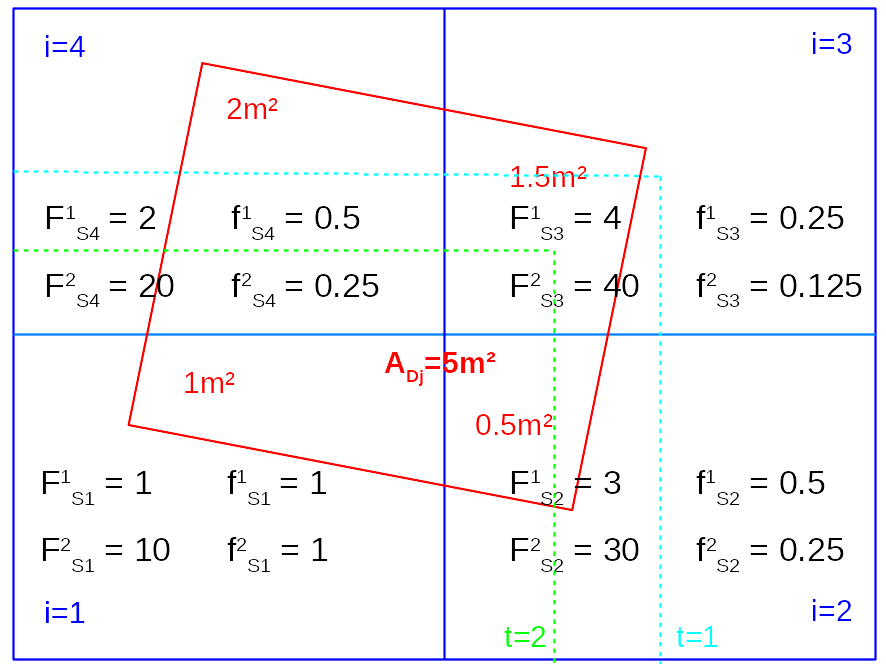
\includegraphics[width=0.75\linewidth]{figures/Fract_interp.png}
    \caption{Source and destination grids for the test case}
    \label{fig:test-case}
\end{figure}
The conservative remapping weights are therefore:\\
\(w_1 = 0.2\); 
\(w_2 = 0.1\);
\(w_3 = 0.3\);
\(w_4 = 0.4\)\\
At time 1, the active source surface covers the following fractions:\\
\(f^{1}_{S1} = 1.0\);
\(f^{1}_{S2} = 0.5\);
\(f^{1}_{S3} = 0.25\);
\(f^{1}_{S4} = 0.5\)\\
and the source fields is:\\
\(F^{1}_{S1} = 1.0\);
\(F^{1}_{S2} = 3.0\);
\(F^{1}_{S3} = 4.0\);
\(F^{1}_{S4} = 2.0\)\\
% Energy leaving source cells at t=1 : 1x1x1 + 3x0.5x0.5 + 4x0.25x1.5 + 2x0.5x2 = 5.25
% Energy leaving source cells at t=2 : 10x1x1 + 30x0.25x0.5 + 40x0.125x1.5 + 20x0.25x2 = 31.25
% Total energy : 36.50
If we neglected the sub-grid fractions, the remapped field at time 1 would be
\[F^{1}_{Dj}=\sum_i{w_iF^1_{Si}}=2.5\]
% 0.2x1 + 0.1x3 + 0.3x4 + 0.4x2 = 2.5
and it's contribution to the integral quantity on the destination grid would be
\[A_{Dj}F^{1}_{Dj}=12.5\]
% 5x2.5 = 12.5
If we take into consideration the source fractions, the destination scaled field as in eqn. (\ref{eqn:inst_scaled}) is
\[F^{1f}_{Dj} = \sum_iw_{i}f^1_{Si}F^1_{Si} = 1.05\]
%  0.2x1x1 + 0.1x0.5x3 + 0.3x0.25x4 + 0.4x0.5x2 = 1.05
It's contribution to the integral quantity on the destination grid is reduced to:
\[A_{Dj}F^{1f}_{Dj} = 5.25\]
% 5x1.05 = 5.25 OK
Taking into consideration the active destination surface coefficients as in eqn. (\ref{eqn:inst_dest_fract})
\[f^1_{Dj} = \sum_i{w_{i}f^1_{Si} = 0.525}\]
% 0.2x1 + 0.1x0.5 + 0.3x0.25 + 0.4x0.5 = 0.525
We can get the destination normalized scaled field as in eqn. (\ref{eqn:normalized_field})
\[F^{1fn}_{Dj} = \frac{F^{1f}_{Dj}}{f^1_{Dj}} = 2.0\]
% 1.05 / 0.525 = 2.0
and the active destination surface as in eqn. (\ref{eqn:active_dest_area})
\[A^{1a}_{Dj} = A_{Dj}f^1_{Dj} = 2.625\]
% 5 x 0.525 = 2.625
and find again the appropriate contribution to the integral quantity on the destination grid
\[A^{1a}_{Dj}F^{1fn}_{Dj} = 5.25\]
% 2.0 x 2.625 = 5.25 OK
\\
Let's now suppose that at time 2, the active source surface covers the following fractions:\\
\(f^{2}_{S1} = 1.0\);
\(f^{2}_{S2} = 0.25\);
\(f^{2}_{S3} = 0.125\);
\(f^{2}_{S4} = 0.25\)\\
and the source fields is:\\
\(F^{2}_{S1} = 10.0\);
\(F^{2}_{S2} = 30.0\);
\(F^{2}_{S3} = 40.0\);
\(F^{2}_{S4} = 20.0\)\\
\\
The instantaneous destination scaled field will then be:
\[F^{2f}_{Dj} = \sum_iw_{i}f^2_{Si}F^2_{Si} = 6.25\]
% 0.2x1x10 + 0.1x0.25x30 + 0.3x0.125x40 + 0.4x0.25x20 = 6.25
It's contribution to the integral quantity:
\[A_{Dj}F^{2f}_{Dj} = 31.25\]
% 5 x 6.25 = 31.25 OK
The active destination surface coefficient:
\[f^2_{Dj} = \sum_i{w_{i}f^2_{Si} = 0.3625}\]
% 0.2x1 + 0.1x0.25 + 0.3x0.125 + 0.4x0.25 = 0.3625
The destination normalized scaled field:
\[F^{2fn}_{Dj} = \frac{F^{2f}_{Dj}}{f^2_{Dj}} = 17.2414\]
% 6.25 / 0.3625 = 17.24137931
and the corresponding active destination surface :
\[A^{2a}_{Dj} = A_{Dj}f^2_{Dj} = 1.8125\]
% 5 x 0.3625 = 1.8125
which confirms the appropriate contribution:
\[A^{2a}_{Dj}F^{2fn}_{Dj} = 31.25\]
% 17.24137931 x 1.8125 = 31.25 OKe
\\
If we accumulate the field on the two time steps, neglecting the sub-grid fractions we obtain\\
\(F^{+}_{S1} = 11.0\);
% 1 + 10 = 11
\(F^{+}_{S2} = 33.0\);
% 3 + 30 = 33
\(F^{+}_{S3} = 44.0\);
% 4 + 40 = 44
\(F^{+}_{S4} = 22.0\)\\
% 2 + 20 = 22
and the destination accumulated field would be (equation \ref{destination_accumulated})
\[F^{+}_{Dj}=\sum_i{w_iF^{+}_{Si}}=27.5\]
% 0.2x11 + 0.1x33 + 0.3x44 + 0.4x22 = 27.5
Meanwhile, if we accumulate the scaled source fields we have\\
\(F^{+f}_{S1} = 11.0\);
% 1x1 + 10x1 = 11
\(F^{+f}_{S2} = 9.0\);
% 3x0.5 + 30x0.25 = 9
\(F^{+f}_{S3} = 6.0\);
% 4x0.25 + 40x0.125 = 6.0
\(F^{+f}_{S4} = 6.0\)\\
% 2x0.5 + 20x0.25 = 6.0
and the destination accumulated scaled field (equation \ref{eqn:nonnorm_accumulate_scaled}) has a much lower value:
\[F^{+f}_{Dj}=\sum_i{w_iF^{+f}_{Si}}=7.3\]
% 0.2x11 + 0.1x9 + 0.3x6 + 0.4x6 = 7.3
It's contribution to the integral quantity on the destination grid is:
\[A_{Dj}F^{+f}_{Dj} = 36.5\]
% 5 x 7.3 = 36.5
\\
We can obtain a more representative value by accumulating the instantaneous normalized scaled fields as in eqn. (\ref{eqn:accumulate_scaled})
\[F^{+fn}_{Dj}=\sum_t{\frac{F^{ft}_{Dj}}{f^t_{Dj}}}=19.24137931\]
% 1.05/0.525 + 6.25/0.3625 = 19.24137931
and derive its equivalent active destination cell fraction from eqn. (\ref{eqn:equivalent_dest_frac})
\[f^+_{Dj} = \frac{F^{+f}_{Dj}}{F^{+fn}_{Dj}} = 0.379390681\]
% 7.3 / 19.24137931 = 0.379390681
and an active surface:
\[A^a_{Dj}=A_{Dj}f^+_{Dj}=1.896953405\]
% 5 x 0.379390681 = 1.896953405
\\
Since the average values are just the half sum of the instantaneous values, the fractions are the same as in the accumulation case.\\
The averaged scaled source fields on the four cells are\\
\(\overline{F}^{f}_{S1} = 5.5\);
% (1x1 + 10x1)/2 = 5.5
\(\overline{F}^{f}_{S2} = 4.5\);
% (3x0.5 + 30x0.25)/2 = 4.5
\(\overline{F}^{f}_{S3} = 3.0\);
% (4x0.25 + 40x0.125)/2 = 3.0
\(\overline{F}^{f}_{S4} = 3.0\)\\
% (2x0.5 + 20x0.25)/2 = 3.0
The scaled remapped field is:
\[\overline{F}^{f}_{Dj}=\sum_i{w_i\overline{F}^{f}_{Si}}=3.65\]
% 0.2x5.5 + 0.1x4.5 + 0.3x3 + 0.4x3 = 3.65
It's contribution to the integral quantity on the destination grid is:
\[A_{Dj}\overline{F}^{f}_{Dj} = 18.25\]
% 5 x 3.65 = 18.25
\\
By averaging the normalized remapped values we obtain the more representative averaged field
\[\overline{F}^{fn}_{Dj}=9.620689655\]
and derive its equivalent active destination cell fraction 
\[\overline{f}_{Dj} = \frac{\overline{F}^{f}_{Dj}}{\overline{F}^{fn}_{Dj}} = 0.379390681\]
which is the same as in the accumulation case and implies an active surface:
\[A^a_{Dj}=A_{Dj}\overline{f}_{Dj}=1.896953405\]


